\chapter{Controller Design}\label{ch:controldesign}
\todo[color=07controllerDesign]{Controller Design not enough text yet}
There exist many different approaches to designing a controller,
all of which have their advantages and disadvantages.
For this project we decided to use a very simple approach,
the Proportional Derivative Integral (PID) controller.
This chapter compares this to another possible option,
the state-space controller, explains both of them briefly
and argues for our choice.

\section{PID control}\label{sec:PID}
A PID controller consists of three parts,
a proportional, integral and derivative part,
which it inherits its name from.
A mathematical representation can be given by one of the two equations in Equation \ref{eq:PID}.

\begin{equation}
	  D_{cl}(s) = k_P + \frac{k_I}{s} + k_D s$$
	$$D_{cl}(s) = k_P ( \frac{T_I}{s} + T_D s)
	 \label{eq:PID}
\end{equation} \cite{Franklin2014}\\
These equations can be visualised in block diagrams, as shown in Figure \ref{fig:twoPID}.
\begin{figure}[H]
    \centering
    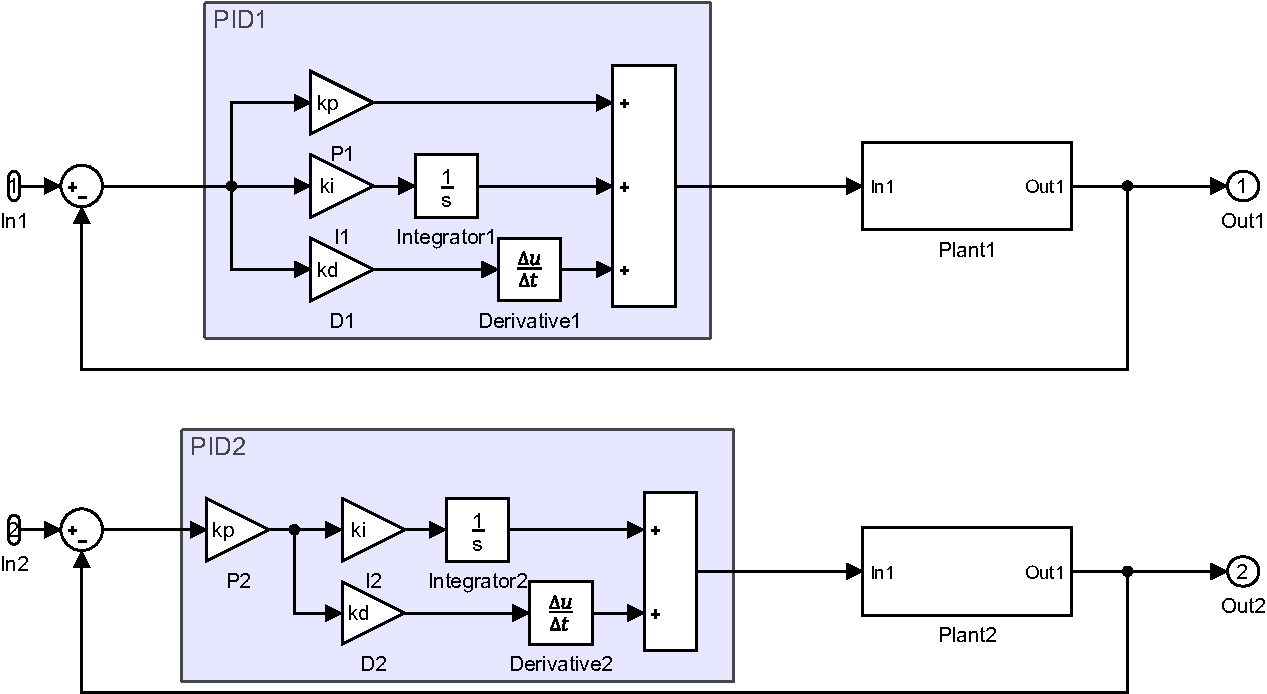
\includegraphics[width=\textwidth]{figures/07controllerDesign/PID_explicit.pdf}
    \caption{Comparison of two common PID designs}
	\label{fig:twoPID}
\end{figure}

Figure \ref{fig:twoPID} also shows the typical placement of a PID-controller,
on the forward loop, behind the subtraction of the feedback and before the input to the plant.

The gains $k_P$, $k_I$ and $k_D$ have to be tuned according to the dynamics of the plant
and the desired characteristics of the controller.
This tuning can be done manually,
\todo[color=07controllerDesign]{find source for manual tuning}
or methodically.
We chose to use the Ziegler-Nichols tuning method,
as described by Franklin et al. \cite{Franklin2014},
as this method promised results inside our requirements and was discussed in our courses.

To use this method, some knowledge about the system is required.
Depending on the stability of the open loop system,
this can be acquired in one of two ways.
If the system reacts stable to a step input,
\todo[color=07controllerDesign]{I think that is wrong, please someone check}
the output measured can be used to tune $k_P$, $k_I$ and $k_D$ according to the "quarter decay method"
\cite{Franklin2014}.

In the case that the system has an unstable reaction,
\todo[color=07controllerDesign]{Then this is also wrong}
the "Ultimate Sensitivity Method" should be used.
Here the $k_p$ is increased until the system becomes marginally stable.

In both cases the output of the system is to be graphed over the time elapsed
and from the corresponding graph some characteristic values can be read.
Because we are using the quarter decay method,
we won't discuss the ultimate sensitivity method any further.

As mentioned before,
to use the QDM, we need a step response of the system.
The following section explains step response in more detail and shows our analysis.

\subsection{Quarter Decay Tuning}
To obtain all needed data,
a step input is to be input into the plant
and the output recorded.
\subsubsection{Step Response}
A block diagram of this setup can be seen in Figure \ref{fig:OL}.
Comparing this figure with \ref{fig:twoPID} highlights
that no feedback or controller is used to observe only the dynamics of the plant.

\begin{figure}[H]
    \centering
    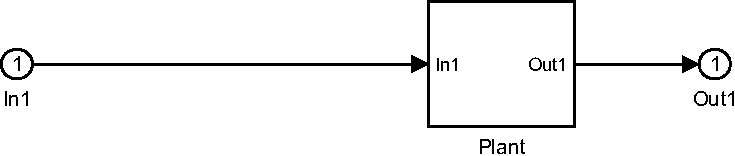
\includegraphics[width=0.75\textwidth]{figures/07controllerDesign/OLblock.pdf}
    \caption{OL block diagram of the system}
\label{fig:OL}
\end{figure}

The recorded output can be seen in Figure \ref{fig:stepin}.
The figure also shows two red lines, approximating the slope and the final value.

\begin{figure}[H]
    \centering
    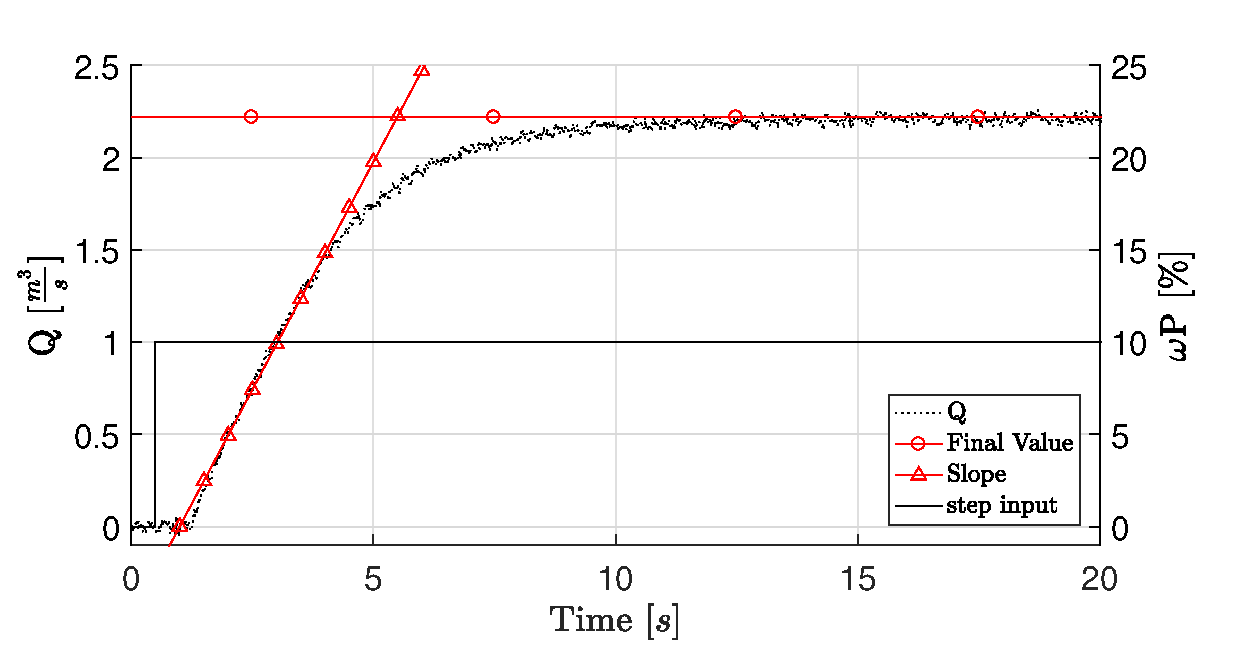
\includegraphics[width=\textwidth]{figures/07controllerDesign/StepResponseLabeled.eps}
    \caption{response to a step input with value 10}
	\label{fig:stepin}
\end{figure}
\todo[color=07controllerDesign]{can we make all axis look like they are made by LaTeX as well?}

From this graph we can approximate the slope $R$ and the Lag $L=t_d$.




Because we are scaling the $\omega$ down by a factor of 10, so we can directly read the percentage,
we had to scale the aforementioned unit step up by a factor of 10,
in order to get usable results.
While encountering this problem, we also noticed, that the pumps don't spin below an $\omega$ of 9\%.
When using the corrected step input, we got the measurements shown in figure X \ref{fig:stepin}.

Our analysis of figure \ref{fig:stepin} gives us the following values:
\\
\begin{tabular}{r c l l}
	$R$ 	& $=$ & $2.0236$ 	& \footnotesize{\textit{slope}}\\
	$t_d=L$	& $=$ & $0.75$ 		& \footnotesize{\textit{lag}}\\
\end{tabular}


\subsubsection{Tuning}
The QDM is tuning a P, PI or PID controller $D_c(s)$ with the formula shown in the second Equation \ref{eq:PID}.
The values of $k_P$, $T_I$ and $T_D$ are scalar gains,
tuned according to the characteristics obtained from figure \ref{fig:stepin}.
\\\\
\begin{tabular}{l r c l l}
	Type of Controller	& \multicolumn{3}{ c }{Optimum Gain}\\
	\hline
	\multirow{1}{*}{P}	& $k_P$ & $=$ & $\nicefrac{1}{RL}$	\\
	\\
	\multirow{2}{*}{PI}	& $k_P$ & $=$ & $\nicefrac{0.9}{RL}$\\
						& $T_I$ & $=$ & $\nicefrac{L}{0.3}$	\\
	\\
	\multirow{3}{*}{PID}& $k_P$ & $=$ & $\nicefrac{1.2}{RL}$\\
						& $T_I$ & $=$ & $2L$				\\
						& $T_D$ & $=$ & $0.5L$ 				\\
\end{tabular}
Note that the parameters $T_I$ and $T_D$ not mentioned for the first two controller types are to be set to 0 and therefore ignored.
\todo[color=07controllerDesign]{Is this table readable?}

\subsubsection{Results}
We tested all three options of P, PI and PID control with the tuned parameters,
the results can be seen in Figure \ref{fig:missing}.

\missingfigure{Comparison of P, PI and PID control}

Unexpectedly, the PID controller settles faster than the other two.
\todo[color=07controllerDesign]{make sure that is true}

One big disadvantage of PID tuning for this system is,
that it is not taking advantage of the existence of three pumps as three individual inputs.
The tuning in this chapter is based on using only a single pump,
but could easily be repeated for multiple pumps with the same input speed.
Based on research done by Pedersen and Yang \cite{YangMultiPump2008},
it seems that using multiple pumps could increase efficiency,
but it be most efficient to always spin all used pumps equally.
This is not possible with a single PID controller,
as it only outputs one speed to all connected pumps.
It could be possible to implement an additional logic,
switching between differently tuned controllers for different flow requirements.

\section{State Space Control}
\todo[color=07controllerDesign]{do we even want that section?}